\documentclass[12pt]{article}
\usepackage{caption}
\usepackage{float}
\usepackage{graphicx}
\usepackage{fancyhdr}
\usepackage[table,xcdraw]{xcolor}
\pagestyle{fancy}
\renewcommand{\headrulewidth}{1pt}
\renewcommand{\footrulewidth}{1pt}
\setlength{\headheight}{10pt}
\rhead{\textbf{Lightning Coalition Robotics}}
\lhead{\textit{FTC Team 9338}}
\cfoot{}
\title{\vspace{-2cm}Table of Contents}
\author{Lightning Coalition Robotics}
\date{January 12, 2019}
\pagenumbering{gobble}
\rfoot{\thepage}
\begin{document}

\maketitle

\section{Summary - Page 1}

\section{About Us - Page 2}

\section{Team Biographies - Page 3}

\section{Engineering Notebook - Page 8}

\section{Website - Page 91}

\section{Parts List - Page 101}

\section{Programming}

\subsection{Autonomous - Page 102}

\subsection{Tele-Op - Page 132}

\subsection{Other - Page 141}

\section{Diagrams and CAD}

\subsection{Arm Designs - Page 150}

\subsection{Drive Train Designs - Page 156}

\subsection{Miscellaneous Designs - Page 158}

\subsection*{}

\newpage
\setlength{\headheight}{25pt}
\setcounter{section}{0}
\pagenumbering{Roman}

\section*{Summary}
In this Engineering Notebook, we explain how our team was created, what happened all throughout the year, and what went together to create our robot in the end. In the \textit{About Us} section, it explains about how the team \textbf{Lightning Coalition Robotics} was originally a family friends team that grew into a team based out of The Key School. In the \textit{Team Biographies} section, we have each member of the team's personal autobiography explaining why they joined the team, what they joined the team, and what they have learned. In the \textit{Engineering Notebook} section, we explain each of our practices in a simple format that gives a reader the plan for the day, then what we got done and what we didn't, then what we plan for next practice. In the \textit{Website} section, we explain how we got a website this year. In the \textit{Parts List} section, we list every part that we have used in our robot this year. In the \textit{Programming} section, we have attached our entire code for our robot. In the \textit{Diagrams and CAD} section, we show all of our drawings and 3D print ideas for the robot. It contains possible and scrapped ideas from this year. We hope you enjoy reading this notebook, thank you.

\newpage
\setcounter{section}{0}

\section*{About Us}
Lightning Coalition Robotics is a fast-growing, student-driven FTC team based out of The Key School in Annapolis. Each year, Lighting Coalition students teach each other about programming, electronic systems, and practical engineering while building a robot to compete in the FTC challenge. Throughout the season, students learn how to think, design, code, and build like engineers.

We started as a family friends coalition in Annapolis in 2014. After a successful rookie year, we became affiliated with The Key School in 2015. This year we were fortunate enough gain two new mentors: one who is an electrical engineer, and another who is a mechanical engineer. They helped broaden our knowledge of computer-aided design (CAD) and organizational flow. We look forward to another successful robotics season competing in Rover Ruckus.

\newpage
\setcounter{section}{0}

\section*{Biographies}

\section{Team Members}

\subsection{Ethan Baker (10th Grade)}
Hi, my name is Ethan Baker, and I was one of the leaders this year. I've been doing FTC for the past two years and before that, I did FLL for four. I like tinkering with parts to get ideas and see how things fit together. Because of that, I did a lot of work on the mechanics of the robot this year.

\subsection{Kenny Casey (9th Grade)}
My name is Kenny Casey, I'm a 9th grader at Keyschool. I was on an FLL team for 6 years, and I recently aged out. I was one of the lead programmers on my FLL team, and I wanted to learn more about programming through FTC.

\subsection{Sarah Celaya (9th Grade)}
I joined robotics because it looked like a fun activity. I liked seeing all the parts come together and problem-solving. I learned that there’s a lot that goes into what looks like a very simple thing and that working with others isn’t as bad as I once thought. 

\subsection{Dylan Donaldson (10th Grade)}
This is my first time joining the robotics team. I joined the team because it seemed very fun and a great experience. I was highly encouraged to join by my peers. Also joining robotics is excellent for my college resume. What I learned was that it takes a lot of teamwork. I also learned how to set up the lunar lander and the course.

\subsection{John Du (10th Grade)}

\subsection{Griffin Dugan (10th Grade)}
I joined the Lightning Coalition Robotics last year because a bunch of my friends were doing it. I really enjoy the aspect of how we have to figure out unique solutions to the problems. I've been leading on the notebook this year, and I've learned the joys of management and the ins and outs of working with a diverse group of people.

\subsection{Anna Estremsky (10th Grade)}
My name is Anna Estremsky. I joined robotics because I have been interested since middle school. I was hesitant at first because I was not sure if it was for me or not. I finally joined this year because my friends convinced me and I thought it would be a fun learning opportunity. I still have a long way to go, but I have gotten a much better understanding of how building and coding a robot works than I had before. I have had a great time hanging out with my friends and learning new things. 

\subsection{Chris Lonergan (10th Grade)}
My name is Christopher Lonergan, I am currently attending The Key School as a sophmore and do a bit of everything, notebook, coding, and building. Over this year, I have tried my best to organize parts for easier access, gain a firm understanding of both Java and the FTC Java API, and I dabbled a small amount with designing things for the robots tasks. I also helped manage the notebook. I really enjoyed working with the team, and look forward to doing this again next year

\subsection{Will Nolan (11th Grade)}
Hello, My name is William Nolan. This is my first year doing FTC, and, so far, I am loving it. I have always enjoyed tinkering with parts salvaged from old electronics and seeing what Frankenstein-like creation I can put together. However, last year, I became interested in the software aspect of technology and have consequently taught myself Python and Java. While I did channel my energy into bug bounty projects, I missed learning about the core mechanics of systems. Therefore, I joined Lightning Coalition robotics, and I’ve had fun working with both the robot’s design and software immensely.

\subsection{Gabe Ruoff (12th Grade)}
My name is Gabe Ruoff. I’m a senior at The Key School and the leader of LC Robotics. This year I’ve worked as a project manager to streamline LC’s development process and have helped my teammates learn how to draft parts and assemblies in CAD, program in Java, and have organized our design and build process. This season, I’ve gained leadership and project management experience by managing the team and its budget, as well as technical experience by building our robot’s chassis and drive chain while writing the autonomous and teleop programs. I’ll be attending university this year to pursue degrees in electrical engineering and music with the hope of specializing in autonomous systems later in my career.

\subsection{Noah Simon (10th Grade)}
My name is Noah Simon, I am a sophomore at The Key School, and I am LCR’s lead programmer. Over the course of the year, I have taught newer members how to use the FTC Java API and implemented processes streamlining collaboration between programmers and simplifying the code-writing process for next season.

I have been participating in FIRST Robotics since sixth grade, when I joined my school’s FLL team. When I aged out of that, I joined LCR and became a mentor to the FLL team. I enjoy engineering, especially software engineering, and I have worked on multiple programming projects outside of robotics.

\subsection{Nathaniel Smith (9th Grade)}
I am Nathaniel Smith and I joined robotics because I have always been interested in invention and creation. The unique obstacles presented by the robot encourage unconventional problem solving. Truly, I have learned much during the process of designing and building the robot.

\subsection{Mimi Whalen (9th Grade)}

\subsection{Zoey Yao (11th Grade)}
Hi my name is Zoey Yao. I’m new to Key school this year, and I actually read about the school robotics team on the website before applying. With some basic knowledge of engineering and coding as well as passion and curiosity, I decided to become part of the robotics team. It’s fun to communicate with teammates because sometimes our ideas and be so different. And getting to know CAD, designing, several coding languages, 3D printers etc helps me to think about what I want in college.

\subsection{Sherry Zhou (10th Grade)}

\section{Coaches}

\subsection{Marissa Gonzalez}
Five years ago my daughter asked me to coach her fledgling robotics team.  She has since graduated and I am still here.  Every year is a new and exciting experience where I watch students grow intellectually as well as socially.   Some of my greatest memories include when my students work together to come to a solution or struggle to break the laws of time and physics.  This is my fun space.

\subsection{Derek Lieskie}
This is my 5th year coaching the robotics team at Key.  I am a physics and astronomy teacher in the Upper School and have enjoyed watching the students take the concepts they learn in class and apply them to their robot. 

\section{Mentors}

\subsection{Craig Casey}
My name is Craig Casey. I am an electrical engineer with over 25 years of professional experience. I have been an FLL coach for the last 6 years and this is my first year mentoring an FTC team. 

\subsection{Mitch Coon}
My name is Mitchell Coon. I recently graduated from the University of Michigan with a Master’s degree in Robotics Engineering. I chose this major because I hope to work on autonomous vehicles in order to prevent car accidents caused by human error. This was my first year working as a mentor for an FTC team.

\newpage
\setcounter{section}{0}

September 8, 2018 - Griffin Dugan

\section{Our Plan:} 
\begin{itemize}
	\item Take notes on the new rules. 
	\item Brainstorm! 
	\item Begin strategizing.
	\item Decide what parts need to be focused on. 
\end{itemize}

As it is the kickoff, we need to watch the challenge video and take it apart. Then we need to begin strategizing and brainstorming. 

\section{What We Got Done:}
\begin{itemize}
	\item Notes were taken on the rules.
	\item Brainstormed! 
	\item Started to strategize. 
	\item Decided what parts needed to be focused on. 
\end{itemize}

When we were taking notes on the rules, some of the rules surprised us, like how there is now a weight limit. This will be interesting as our robot was very heavy last year. Then, we decided to think about what to focus on for the competition. The latching and detaching to the hooks seem to be very important as one can get 75 points by doing both. From this, we decided that we need to figure out how to connect our robot to the hook. We thought that we should raise up a hook and attach to the hook in the center, then we would raise up the robot. 

\section{What We Didn't Get Done:} 
\begin{itemize}
	\item Nothing! 
\end{itemize}

As it was only the kickoff, we weren't able to have much to do except brainstorm. 

\section{Next Practice:}
\begin{itemize}
	\item Fully take apart the challenge. 
	\item Start planning. 
	\item Decide how we are going to work this year. 
\end{itemize}

The next practice is currently unknown as we haven't had a full meeting yet. Even so, we will want to fully take apart the challenge and gather what things give us points. We will want to start planning. After that, we will want to decide how we will work this year buy deciding what things need to be done and what will take the most time.

\newpage
\setcounter{section}{0}

September 13th, 2018 - Griffin Dugan


\section{Our Plan:}
\begin{itemize}
	\item Introduce the team.
	\item Help out the new people.
	\item Brainstorm!
\end{itemize}

Our plan for today is to get the team started and working together. Since we have a bunch of new people on the team, we need to get them understanding the FTC system. Also, we need to do some brainstorming.

\section{What we did:}
\begin{itemize}
	\item Introduced the team.
	\item Helped out new people.
\end{itemize}

We started out the practice by introducing the team to everyone else. Then we watched the FTC challenge video so that we understood what we would have to do. Then we made a rough plan for this season. After that, we left it open to the new team members to ask questions about FTC and the challenge.

\section{What we didn't do:}
\begin{itemize}
	\item Brainstorm...
\end{itemize}

The questions from the new team members took longer than we had expected, so we weren't able to start brainstorming. 

\section{Next Practice:}
\begin{itemize}
	\item Make a plan for practices.
	\item Isolate the parts that we should focus on.
	\item BRAINSTORM!
	\item Start building/coding.
\end{itemize}

Our next practice is on Friday the 21st of September. Next week, we want to create a plan for all of the practices that will happen outside of school. Then we want to isolate the certain parts of the challenge that we can work on; this will help as build the robot quicker. After that, we want to finally get around to brainstorming. And hopefully, we want to get around to starting to build and code.

\newpage
\setcounter{section}{0}

September 21st, 2018 - Griffin Dugan

\section{Our Plan:}
\begin{itemize}
	\item Explain notebook
	\item Brainstorm.
\end{itemize}



\section{What We Got Done:}
\begin{itemize}
	\item Explain notebook
	\item Brainstorm.
	\item Create a schedule for notebook.
\end{itemize}



\section{What We Didn't Get Done:}
\begin{itemize}
	\item Nothing!
\end{itemize}



\section{Next Practice:}
\begin{itemize}
	\item Start on the robot.
	\item Brainstorm some more.
\end{itemize}

The next practice is Saturday, September 22nd, 2018.

\newpage
\setcounter{section}{0}

September 22nd, 2018 - Chris Lonergan

\section{To Start:}
We first went over the basic parts of the robot (Core Motor Controller, Core Power Distribution Module, chassis, ect.) After that, we watched the FTC video on the competition to gauge our objectives this year. 

\section{Specifying Requirements:}
We realized that there were certain parameters that our robot needed to fulfill. 
\begin{itemize}
	\item 18x18x18 inches Cubed
	\item 8 Motors max
	\item 42 lb max
\end{itemize}

\section{Divide And Conquer:}
Next, we separated our team into four groups: Chassis and Drive Chain, Lifting and Lowering Robot, Autonomous, and Blocks and Balls.

\subsection{Chassis and Drive Chain:}
The Chassis and Drive Chain group decided that the best method was a tank drive, a triangular shape that uses treads instead of wheels. 
This design would be able to incorporate the drawer slide and shovel ideas from the other groups as well. It would also serve as an easier method for climbing over the sides of the crater, as the treads are built for terrain.

\subsection{Lifting and Lowering Robot:}
The lifting and Lowering Robot group decided on using a drawer slide to lift the robot off of the ground. It will be at the center of gravity so that the robot can lift vertically without falling over. 

\subsection{Autonomous:}
The autonomous group made a flow chart of the program that the robot will need to follow. It outlined all of the steps we need to take in the Autonomous section and how many points each objective is worth.

\subsection{Blocks and Balls:}
An important part of the mission is gathering materials and moving them around. The group had several ideas.
\begin{itemize}
	\item Launching 
	\item Arm/Claw
	\item Shovel
\end{itemize}
The idea of launching balls was quickly discarded, as it is inaccurate and could be unsafe. The arm/claw idea was designed for the square minerals, as if we put 4 'fingers' on the arms it could grab the square by the edges and firmly grasp it. The other idea was a shovel. The shovel would be thin and scoop up the materials, but only have room for two materials, so that we do not accidentally pick up three at once, which would be against the rules.

\section{Wrapping Up:}
To end our practice, all the groups came together and shared their ideas and designs with everyone else. We set up a schedule for practices and brainstormed as a group to fine tune several of our ideas. The notebook group also tried to lay out and organize a system for the notebook, and introduced the newer members to LaTex, the programming language we are using for notebook.

\newpage
\setcounter{section}{0}

% Add date (e.g. September 14, 2018) and then your name/all authors.
9/29/18 - Anna Estremsky

\section{Our Plan:} % Pretty self explanatory... In this section explain the team's plan.
\begin{itemize}
% After \item, add what you want for the bullet point. (\item adds a new bullet point when you run out.)
	\item learn python/java
\item fix 3-D printer
\item organize materials
\end{itemize}

% Now add a paragraph explaining your plan. You should reference the bullet points above.
Our plan was fairly simple. We had three main goals: teaching python and or java to those interested in coding, fixing the 3-D printer, and organizing materials.  

\section{What We Got Done:} % Just like the above, explain what the team got done during practice.
\begin{itemize}
% After \item, add what you want for the bullet point. (\item adds a new bullet point when you run out.)
	\item learned some java
\item fixed 3-D printer
\item downloaded solidworks
\item tutorial on android studio
\item organized materials
\item ordered field
\item worked on tank drive

\end{itemize}

% Now add a paragraph explaining what you got done and the reasons behind it. You should reference the bullet points above.
It was a Saturday so we were able to get plenty of things done. We ordered the field so we can start assembling it when it arrives. Those who planned to work with solidworks downloaded that. We were shown the basics of how to operate Android Studio. A few of us continued organizing materials.The 3-D printer was fixed. Some people also worked on the tank drive.

\section{What We Didn't Get Done:} % Explain what the team didn't get done during practice.
\begin{itemize}
% After \item, add what you want for the bullet point. (\item adds a new bullet point when you run out.)
	\item learn python
\end{itemize}

% Now add a paragraph explaining what you didn't get done and the reasons behind it. You should reference the bullet points above.
Since our plan only involved a few things, there wasn’t anything that needed to be done that wasn’t. We did not teach any python because the people who were interested in coding already knew it. We did not completely finish organizing materials because that is a large job, but we made good progress. 

\section{Next Practice:}
\begin{itemize}
% After \item, add what you want for the bullet point. (\item adds a new bullet point when you run out.)
	\item nothing to report
\end{itemize}

% Now add a paragraph explaining what the plan for next practice should be. You should reference the bullet points above.
The next practice is 10/5/18. Next practice is a Friday so we do not have a plan. We will do what we can in the limited time.

\newpage
\setcounter{section}{0}

% Add date (e.g. September 14, 2018) and then your name/all authors.
October 5, 2018 - Noah Simon

\section{Our Plan:} % Pretty self explainatory... In this section explain the team's plan.
\begin{itemize}
% After \item, add what you want for the bullet point. (\item adds a new bullet point when you run out.)
	\item Unpack Stuff
	\item Take inventory
	\item Get coding infrastructure set up on members' computers
\end{itemize}

% Now add a paragraph explaining your plan. You should reference the bullet points above.
We just got our shipments in, including both board- and robot-building materials. We need to take all that out, and make sure we have everything that we're supposed to have. Also, we need to get Android Studio set up on all the coders' computers. 

\section{What We Got Done:} % Just like the above, explain what the team got done during practice.
\begin{itemize}
% After \item, add what you want for the bullet point. (\item adds a new bullet point when you run out.)
	\item Unpack Stuff
	\item Take inventory
	\item Ideas for claw mechanism
\end{itemize}

% Now add a paragraph explaining what you got done and the reasons behind it. You should reference the bullet points above.
We basically dumped everything out on the floor, and figured out what we have. It turns out we are missing all of the lander materials due to a backorder. Nothing we can do about that except wait. We also messed around with different ways to construct a claw mechanism for picking up scoring elements.

\section{What We Didn't Get Done:} % Explain what the team didn't get done during practice.
\begin{itemize}
% After \item, add what you want for the bullet point. (\item adds a new bullet point when you run out.)
	\item Get coding infrastructure set up on member's computers.
\end{itemize}

% Now add a paragraph explaining what you didn't get done and the reasons behind it. You should reference the bullet points above.
This was a short practice, only 45 minutes, so we weren't expecting to get too much done with regards to actually building things. However, how hard can setting up Android Studio be? It turns out: very difficult. Android Studio is already complicated to set up, and this was exacerbated by our school's incredibly slow WiFi connection. 

\section{Next Practice:}
\begin{itemize}
% After \item, add what you want for the bullet point. (\item adds a new bullet point when you run out.)
	\item Finish setting up coding infrastructure
	\item Start building a chassis
	\item Inventory motors, servos, etc.
	\item Order any of the above items we need
\end{itemize}

% Now add a paragraph explaining what the plan for next practice should be. You should reference the bullet points above.
The next practice is tomorrow, October 6. % And then continue the paragraph.
Four hours tomorrow should hopefully be enough time for our lead programmer to get the development environment set up for everyone. The builders can finally start actually building since we have a better idea of what we are building for. We also should take a look at how many hardware components we have and see if we need to order more.

\newpage
\setcounter{section}{0}

% Add date (e.g. September 14, 2018) and then your name/all authors.
10/6/18 - Anna Estremsky

\section{Our Plan:} % Pretty self explanatory... In this section explain the team's plan.
\begin{itemize}
% After \item, add what you want for the bullet point. (\item adds a new bullet point when you run out.)
	\item organizing materials
	\item play with ideas
	\item learn java

\end{itemize}

% Now add a paragraph explaining your plan. You should reference the bullet points above.
We planned to continue working out some ideas on how to accomplish our task. We also wanted to work on organizing parts. People who already knew some python planned to work on learning some java. 

\section{What We Got Done:} % Just like the above, explain what the team got done during practice.
\begin{itemize}
% After \item, add what you want for the bullet point. (\item adds a new bullet point when you run out.)
	\item continued organizing materials
	\item worked on possible designs 
	\item learning java

\end{itemize}

% Now add a paragraph explaining what you got done and the reasons behind it. You should reference the bullet points above.
Today we continued to organize materials because there were a lot that needed to be sorted out, and only a few people were doing this. We spent some time planning and sketching ideas for various functions of the robot. A few people who were interested in coding and already knew how to use python stepped out of the room to be taught how to code in java. 

\section{What We Didn't Get Done:} % Explain what the team didn't get done during practice.
\begin{itemize}
% After \item, add what you want for the bullet point. (\item adds a new bullet point when you run out.)
	\item nothing to report
\end{itemize}

% Now add a paragraph explaining what you didn't get done and the reasons behind it. You should reference the bullet points above.
We didn’t have a lot in our plan so there isn’t much to say here.
\section{Next Practice:}
\begin{itemize}
% After \item, add what you want for the bullet point. (\item adds a new bullet point when you run out.)
	\item unknown
\end{itemize}

% Now add a paragraph explaining what the plan for next practice should be. You should reference the bullet points above.
The next practice is 10/13/18. 

\newpage
\setcounter{section}{0}

October 13 - Chris Lonergan

\section{Our Plan:} 
\begin{itemize}
% After \item, add what you want for the bullet point. (\item adds a new bullet point when you run out.)
	\item Drive Chain
	\item Arm
	\item Design mechanism to pick minerals off the ground
\end{itemize}

We wanted to do the tank treads, and test them as well. We also wanted to design a mechanism for our arm that picks the robot up and we wanted to design a mechanism to pick "minerals" off the ground. 

\section{What We Got Done:} 

Today, we assembled the tank treads and tested them. We also designed a worm gear assembly and created a motor CAD file for the robot assembly. 


\section{What We Didn't Get Done:} 

We were unable to fully design a mechanism to pick up minerals.

\section{Next Practice:}
Design the mechanism to pick up "minerals" and create a CAD file for that mechanism.

\newpage
\setcounter{section}{0}

% Add date (e.g. September 14, 2018) and then your name/all authors.
10/19/18 - Anna Estremsky

\section{Our Plan:} % Pretty self explanatory... In this section explain the team's plan.
\begin{itemize}
% After \item, add what you want for the bullet point. (\item adds a new bullet point when you run out.)
	\item discuss plans
\end{itemize}

% Now add a paragraph explaining your plan. You should reference the bullet points above.
We did not have much of a plan for this practice because we only meet for a short time on Fridays. We wanted to figure out how we are going to handle job distribution and the basis of how we will accomplish our main task.

\section{What We Got Done:} % Just like the above, explain what the team got done during practice.
\begin{itemize}
% After \item, add what you want for the bullet point. (\item adds a new bullet point when you run out.)
	\item organize materials	
\end{itemize}

% Now add a paragraph explaining what you got done and the reasons behind it. You should reference the bullet points above.
This was a short practic, so we didn’t do much. We made a little progress organizing and counting materials, but not significant. A few people counted materials to record the inventory. We mostly discussed our plans and how to best carry them out.

\section{What We Didn't Get Done:} % Explain what the team didn't get done during practice.
\begin{itemize}
% After \item, add what you want for the bullet point. (\item adds a new bullet point when you run out.)
	\item nothing to report
\end{itemize}

% Now add a paragraph explaining what you didn't get done and the reasons behind it. You should reference the bullet points above.
Since we didn’t have much of a distinct plan, basically just to do what we can in the short time, there was not anything left to be desired. 

\section{Next Practice:}
\begin{itemize}
% After \item, add what you want for the bullet point. (\item adds a new bullet point when you run out.)
	\item unknown
\end{itemize}

% Now add a paragraph explaining what the plan for next practice should be. You should reference the bullet points above.
The next practice is 10/25/18. We do not have a specific plan in mind yet. 

\newpage
\setcounter{section}{0}

October 25 2018 - William Nolan

\section{Our Plan:} % Pretty self explainatory... In this section explain the team's plan.
\begin{itemize}
% After \item, add what you want for the bullet point. (\item adds a new bullet point when you run out.)
    \item In the beginning, two groups were formed.  The first group focused on assembling the robot testing enviroment, and the second began work on the robot's claw.
    \item Group 1 began with inventorying all of the part of the robot's enviroment.  They put together the central box frame, but couldn't complete it due to the fact that we didn't have the right tools to screw in the nylon hex nuts.
    \item Group 2 decided to break into individuals, and each design their own ideal prototype robot claw. Afterwards they would debate the merits of their designs.
    \item Gabriel Ruoff worked independently to build the robot's chasis and a side tank tread wheel. This was completed.
\end{itemize}

% Now add a paragraph explaining your plan. You should reference the bullet points above.
After about 20 minutes, Group 2 was to come back together and discuss the final design of the robot.

\section{What We Got Done:} % Just like the above, explain what the team got done during practice.
\begin{itemize}
% After \item, add what you want for the bullet point. (\item adds a new bullet point when you run out.)
    \item Group 1 inventoryed all of the materials delivered that were not going to be part of the robot. They completed the intial box for the lander in the Robo Ruckus Course.
    \item Group 2's individual designed their own prototype claw and attachments to the robot and began debated their designs.  For example, Griffin designed a type of ground device which would used high-speed wheels to pick up items.
\end{itemize}

% Now add a paragraph explaining what you got done and the reasons behind it. You should reference the bullet points above.

\section{What We Didn't Get Done:} % Explain what the team didn't get done during practice.
\begin{itemize}
% After \item, add what you want for the bullet point. (\item adds a new bullet point when you run out.)
    \item As I said before, in the second bullet point, Group 1 was unable to finish the robot enviroment.  Hopefully, a charged dremel and a more precise drill bits will allow for greater progress. 
    \item There was no actual resolution with Group 2.  They each designed a device to obtain items from the ground, but they did not have enough time to determine the best one to implement in our robot.
\end{itemize}

% Now add a paragraph explaining what you didn't get done and the reasons behind it. You should reference the bullet points above.
There wasn't enough time for there to be enough discussion to fully decide on the type of claw to implement on the robot.

\section{Next Practice:}
\begin{itemize}
% After \item, add what you want for the bullet point. (\item adds a new bullet point when you run out.)
    \item All in all, while the strategy of how the course is to be handed was not talked about, the time was very productive and the robot's prototype is nearing completion.  
\end{itemize}

% Now add a paragraph explaining what the plan for next practice should be. You should reference the bullet points above.
The next practice is November 2, 2018.  Then, the team plans to finalize the design of the robot's attachments.

\newpage
\setcounter{section}{0}

November 2, 2018 - Dylan Donaldson

\section{Our Plan:} % Pretty self explanatory... In this section explain the team's plan.
\begin{itemize}
% After \item, add what you want for the bullet point. (\item adds a new bullet point when you run out.)
	\item Move items to one room to another at the beginning of class
	\item Continuing to assemble lunar lander
	\item Continuing to assemble the arm

\end{itemize}

% Now add a paragraph explaining your plan. You should reference the bullet points above.
On this day, we had to move items to another room which was Ms. Portifields room. Once the team got settled, a group was continuing to assemble the lunar lander. Dylan, Anna, Sarah, and Mimi were assembling the lunar lander.  Another group was continuing to assemble the arm. Sherry and Zoe were the ones that were assembling the arm.  

\section{What We Got Done:} % Just like the above, explain what the team got done during practice.
\begin{itemize}
% After \item, add what you want for the bullet point. (\item adds a new bullet point when you run out.)
	\item We did not get anything done, because this day was hectic because we had to move to another room.
\end{itemize}

% Now add a paragraph explaining what you got done and the reasons behind it. You should reference the bullet points above.
Nothing got done. Since the next day was an open house for the school, we decided to show off the robotics to the visitors and explain how robotics isn't just about the mechanical side of things, it also has a networking side.
\section{What We Didn't Get Done:} % Explain what the team didn't get done during practice.
\begin{itemize}
% After \item, add what you want for the bullet point. (\item adds a new bullet point when you run out.)
	\item Did not finish assembling the lunar lander
	\item Did not finish assembling the arm
\end{itemize}

% Now add a paragraph explaining what you didn't get done and the reasons behind it. You should reference the bullet points above.

We did not finish assembling the lunar lander and the arm because we had to move to  another room. 

\section{Next Practice:}
\begin{itemize}
% After \item, add what you want for the bullet point. (\item adds a new bullet point when you run out.)
	\item Finish lander
	\item Finish arm
	\item Build the course
\end{itemize}

% Now add a paragraph explaining what the plan for next practice should be. You should reference the bullet points above.
% And then continue the paragraph.. 
The next practice is Thursday, November 3rd, 2018. Our plan for next class is to finish the lunar lander and the arm. Then our next plan is to build the course for the robot. 

\newpage
\setcounter{section}{0}

11/3/2018 - Nathaniel Smith 

\section{Our Plan:} % Pretty self explanatory... In this section explain the team's plan.
\begin{itemize}
% After \item, add what you want for the bullet point. (\item adds a new bullet point when you run out.)
	\item Work on the multiple prototypes for collection mechanisms
	\item Work on the arena, specifically the lander
\item Some of our team learned and began to practice coding so that we will be better equipped when we reach the coding step
\item Work on building the chassis so that we will eventually be able to drive and attach appendages to it
\end{itemize}

% Now add a paragraph explaining your plan. You should reference the bullet points above.
Our plan is to continue working in the chassis because the chassis is one of the most essential parts of the robot. We also plan to continue working on the arena so that we will be able to test our robot in it and get a sense of what coding we need to do and how effective the robot will be. In addition, it is ideal for us to work on multiple prototypes for the collection mechanism so that we will be able to test them and pick which one we like best. Some of us will also learn to code so we can have more members that can work on coding when we get to that step.

\section{What We Got Done:} % Just like the above, explain what the team got done during practice.
\begin{itemize}
% After \item, add what you want for the bullet point. (\item adds a new bullet point when you run out.)
	\item Work on the multiple prototypes for collection mechanisms
	\item Work on the arena, specifically the lander
\item Some of our team learned and began to practice coding so that we will be better equipped when we reach the coding step
\item Work on building the chassis so that we will eventually be able to drive and attach appendages to it
\end{itemize}

% Now add a paragraph explaining what you got done and the reasons behind it. You should reference the bullet points above.
We worked on building the rover ruckus arena so that when it is completed, we can test our robot in it. We also worked on drafting prototypes for collection mechanisms so that when they are complete they can be tested and we will be able to decide which mechanism to use on our robot. Several of our members learned and began to practice coding so that moving forward, we will be advantaged when we reach the coding step. We worked on the chassis so that we can test different attachments on it and practice driving it. We also discussed the car washer and claw mechanisms to compare them so we will have a better idea of the pros and cons of each.

\section{What We Didn't Get Done:} % Explain what the team didn't get done during practice.
\begin{itemize}
% After \item, add what you want for the bullet point. (\item adds a new bullet point when you run out.)
	\item We did not finish the arena.
\end{itemize}

% Now add a paragraph explaining what you didn't get done and the reasons behind it. You should reference the bullet points above.
We were not able to finish the arena, which would have been amazing. Our members working on the arena could not finish it because of problems with the tools and the parts used to construct the arena. Most of the things we planned to do we finished.

\section{Next Practice:}
\begin{itemize}
% After \item, add what you want for the bullet point. (\item adds a new bullet point when you run out.)
\item Work on arena
\item Continue working on the collection mechanism prototypes and hopefully decide what to use
\item Work on the mechanism to lift the robot
\end{itemize}

% Now add a paragraph explaining what the plan for next practice should be. You should reference the bullet points above.
The next practice is, November 8th, 2018. % And then continue*
We want to work on the arena in the next practice because once we finish it, we can test our robot in it. We would also like to continue working on the collection mechanism because once we finish them we can debate their usefulness and decide which to use. It would be ideal to make progress on the mechanism to lift the robot so we can test it.

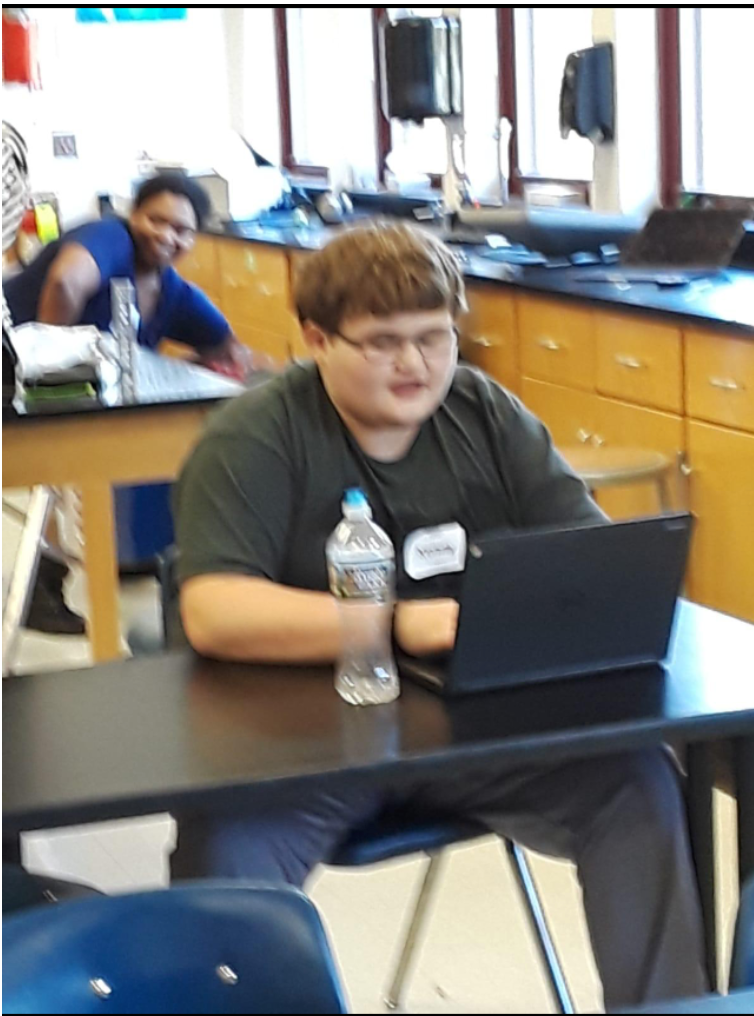
\includegraphics[width=75mm,scale=0.5]{november3/pic1.png}
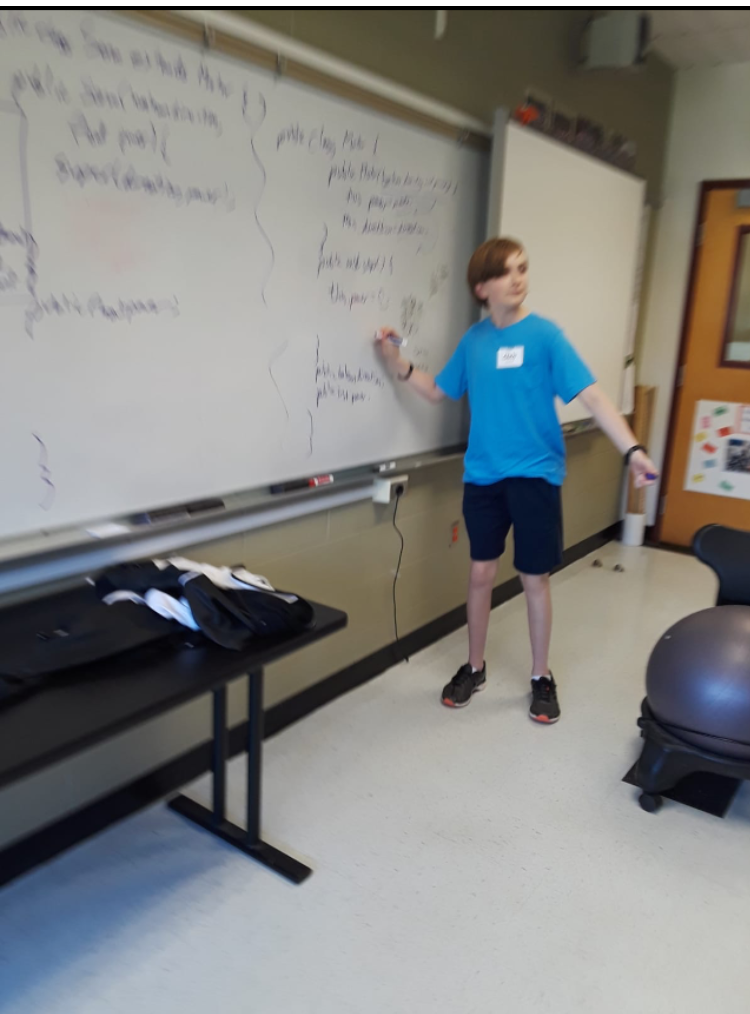
\includegraphics[width=75mm,scale=0.5]{november3/pic2.png}
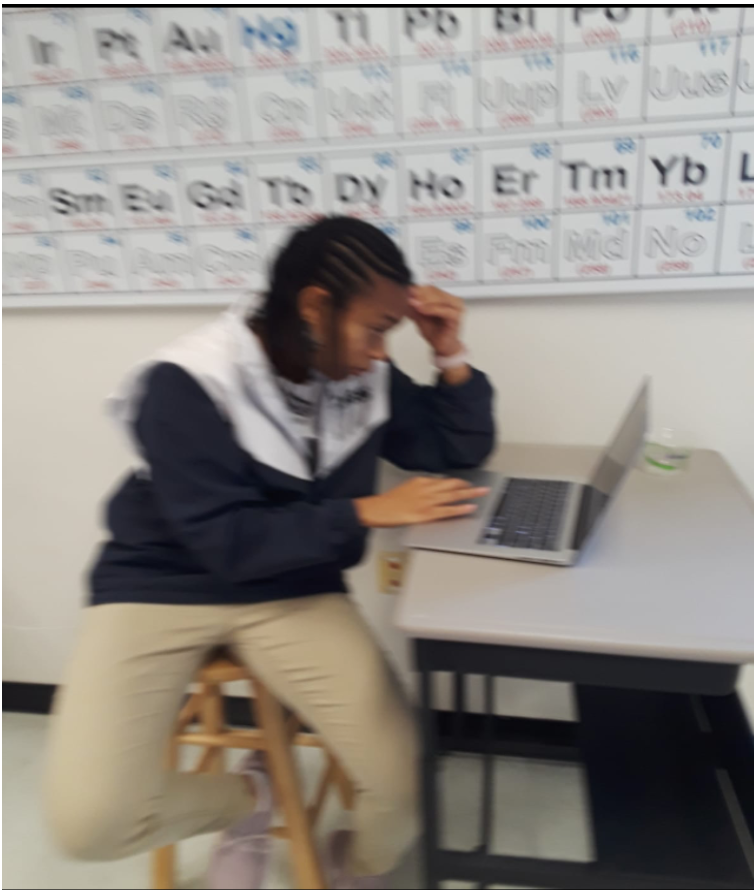
\includegraphics[width=75mm,scale=0.5]{november3/pic3.png}
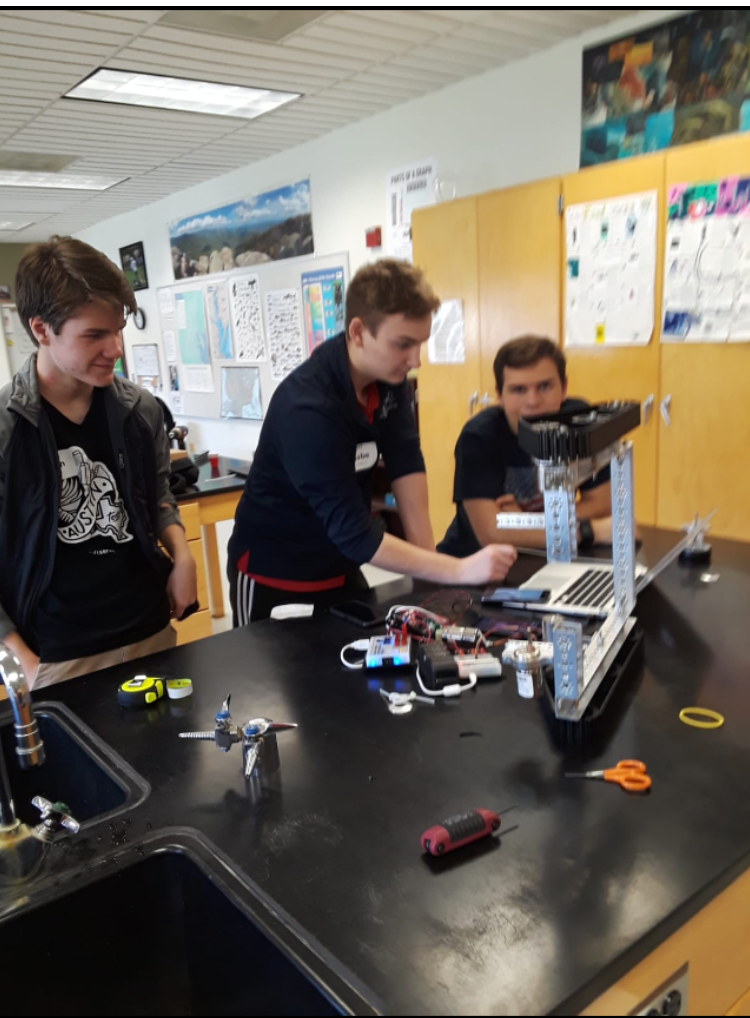
\includegraphics[width=75mm,scale=0.5]{november3/pic4.png}
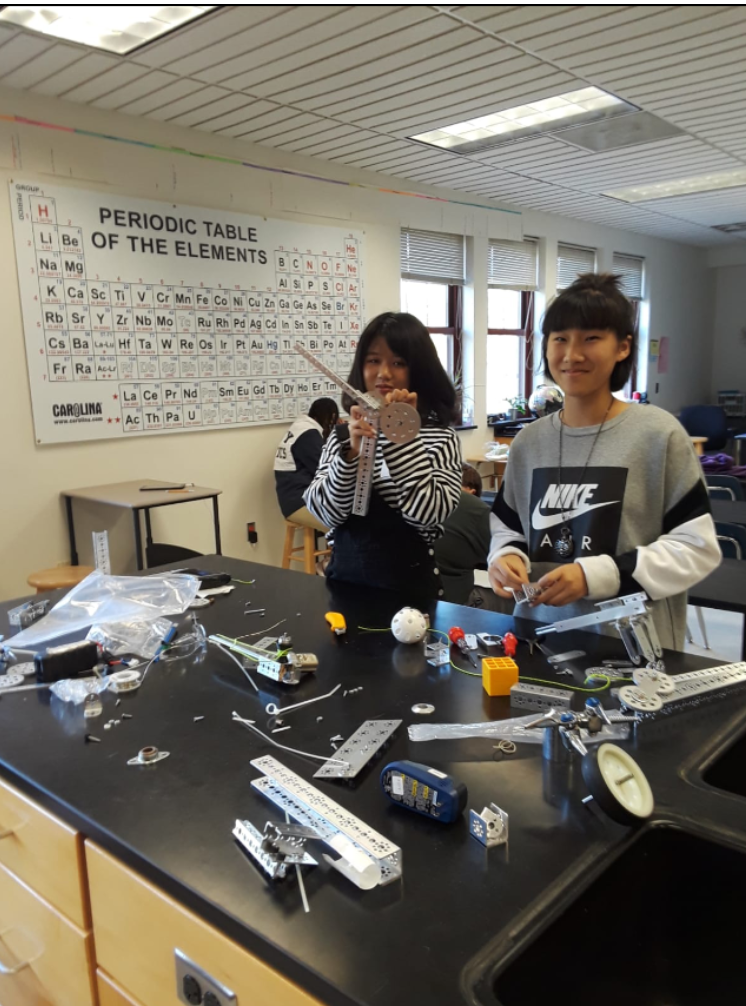
\includegraphics[width=75mm,scale=0.5]{november3/pic5.png}
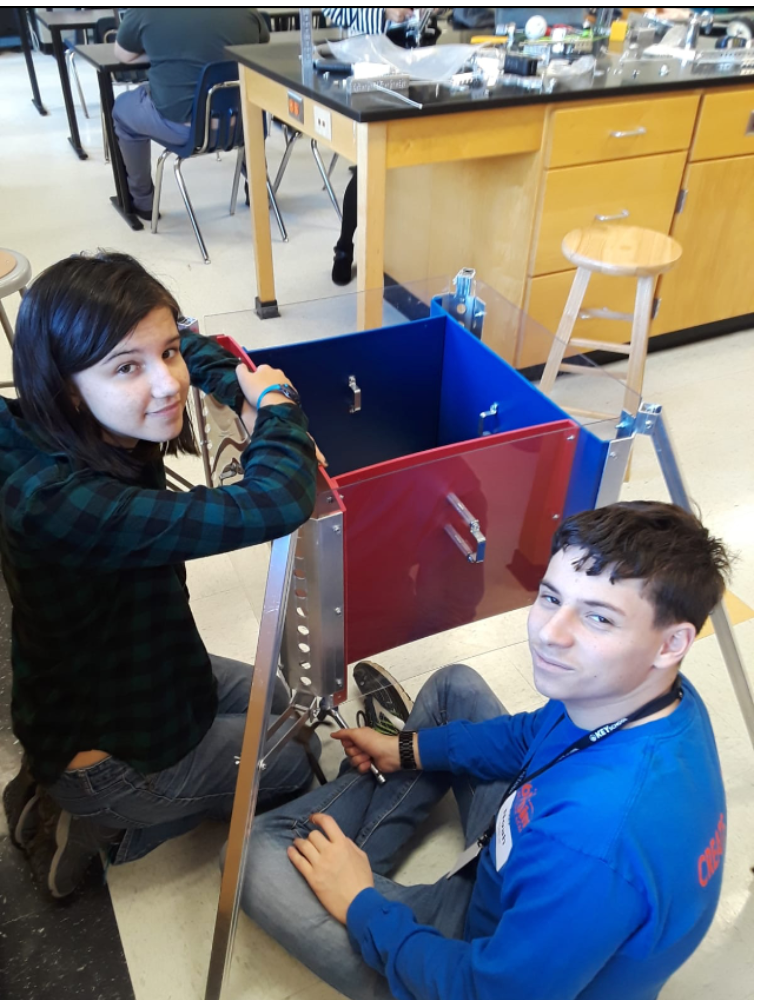
\includegraphics[width=75mm,scale=0.5]{november3/pic6.png}

\newpage
\setcounter{section}{0}

% Add date (e.g. September 14, 2018) and then your name/all authors.
November 8, 2018 - Mimi Whalen

\section{Our Plan:} % Pretty self explanatory... In this section explain the team's plan.
\begin{itemize}
% After \item, add what you want for the bullet point. (\item adds a new bullet point when you run out.)
	\item Work on the lander and it is to finish it by the end of November
	\item Starting to work on different arms for robot
\item 3D Printing
\item CAD
\end{itemize}

% Now add a paragraph explaining your plan. You should reference the bullet points above.
Our plan for today was to get working on the lander and start working on arms to attach to the robot. We needed to get it done before we can begin testing the robot on the course to see how it is moving on the mats. People worked on different arms that would be able to pick up blocks and spares in the crater. There are also some people that started working on put pieces together on CAD and 3D printing those objects.

\section{What We Got Done:} % Just like the above, explain what the team got done during practice.
\begin{itemize}
% After \item, add what you want for the bullet point. (\item adds a new bullet point when you run out.)
	\item One of the arms 
	\item Set date for when the lander should be ready
	\item Some of the 3D printing
\end{itemize}

% Now add a paragraph explaining what you got done and the reasons behind it. You should reference the bullet points above.

We got the base of the lander and the base legs of the lander done. Got the bottom base of the robot and some of the cords to test the robot done. We started printing some parts to add to the robot.

\section{What We Didn't Get Done:} % Explain what the team didn't get done during practice.
\begin{itemize}
% After \item, add what you want for the bullet point. (\item adds a new bullet point when you run out.)
	\item Lander
\item Arms for robot
\item 3D printing
\end{itemize}

% Now add a paragraph explaining what you didn't get done and the reasons behind it. You should reference the bullet points above.
We still have to work out the legs of the lander and put the course together. We got some of the 3D printing done but still have some more 3D printing to do on the arms. We should have both the lander and the 3D printing done by next practice.

\section{Next Practice:}
\begin{itemize}
% After \item, add what you want for the bullet point. (\item adds a new bullet point when you run out.)
	\item Work on the lander and course
\item Work on arms to attach to robot
\item Find a way to lift the robot up and down from the lander 
\end{itemize}

% Now add a paragraph explaining what the plan for next practice should be. You should reference the bullet points above.
The next practice is on November 9, 2018. We will be working trying to finish the lander and start tape out the course. Most of the group will be working on alternative arm options and finding parts to add to the robot. A small group of people started to work on the way to lift the robot off and on the lander.

\newpage
\setcounter{section}{0}

November 9th - Chris Lonergan

\section{Our Plan:} 
\begin{itemize}
% After \item, add what you want for the bullet point. (\item adds a new bullet point when you run out.)
	\item Finish designing and brainstorming mechanism to get balls and blocks into  
	\item Print out a stability test with a new printer filament (TCP)
\end{itemize}

We wanted to fully complete the design of the arm we will be using to pick up the blocks and balls and storing them. We had 3 designs but none of them were fully tested and they each have major flaws.

\section{What We Got Done:} 

We managed to print a test with the new TCP filament in the shape of a boat. This filament was for use in one of the designs we are thinking about using to pick up blocks and balls.

\section{What We Didn't Get Done:} 

We were not able to finish designing all of our options for our arm.

\section{Next Practice:}

Next practice, we want to finish designing our arm mechanisms, and try to figure out which one would be most effective. As well as that, we would like to continue working on coding the autonomous portion of the robot, as well as quality check that every part of the robot is working as it should.

\newpage
\setcounter{section}{0}

November 30 - Gabe Ruoff

\section{Our Plan:}
\begin{itemize}
% After \item, add what you want for the bullet point. (\item adds a new bullet point when you run out.)
	\item Resolve bugs in autonomous code causing the bot to not go straight.
	\item Fix error deviation issues between big and small encoders.
\end{itemize}

We wanted to fix tuning issues with the encoders and the robot's drive function. Thinking that the difference in error distributions between the two encoders' outputs was to blame, we wanted to scale the error of the more precise one up to the error of the less procise one.

\section{What We Got Done:}

We scaled up the error, causing the robot to drive pretty much straight.

\section{What We Didn't Get Done:}

We didn't get the robot driving perfectly straight and still had some minor errors.

\section{Next Practice:}

Swap the small encoder for a second big encoder so that both sides of the drive chain are working with the same encoder system. Should resolve our lingering straightness issues.

\newpage
\setcounter{section}{0}

December 8, 2018 - Griffin Dugan

\section{Our Plan:} 
\begin{itemize}
	\item Choose a collection method.
	\item Add arms to the robot.
	\item Clean up wires on the robot.
	\item Get robot's driving methods fixed.
\end{itemize}

We plan to choose which type of collection method. Then we plan to add the collection method to the robot along with all the other arms. We want to clean up the wires on the robot. Then we also want to get our robot's autonomous driving fixed as it has a few errors currently.

\section{What We Got Done:} 
\begin{itemize}
	\item Figured out which type of collection method we would use.
	\item Re-arranged arm to make it better
	\item Got android studio working for everyone
	\item Added the pull up arm to the robot
	\item Chose a collection method.
	\item Cleaned up wires on the robot.
\end{itemize}

Today, we managed to figure out which collection method we would use. We chose our street washing design, where two wheels spin and pull in the blocks. We also re-arranged the arm to be more compact and less heavy as we may add it later on. We also got android studio working for everyone on the team -- or so we hope. We added the pull up arm onto the robot. So now we have a pulling up mechanism. We also cleaned up the wires on our robot. It's much neater now.

\section{What We Didn't Get Done:}
\begin{itemize}
	\item Get robot's driving methods fixed.
\end{itemize}

The only thing we didn't get done was fix the robot's autonomous driving. We think the problem is something with the length data in the code, so we need to give time to work on it so that we can fix it. It drives fine, except for the fact that it sometimes turns much too much.

\section{Next Practice:}
\begin{itemize}
	\item Get robot's driving methods fixed.
	\item Fully fix up the collection method.
	\item Finish autonomous.
\end{itemize}

The next practice is Saturday, December 15th, 2018.
Next practice, we plan to get the robot's autonomous finished. This includes fixing the robot's autonomous driving. Also, we need to fully finish adding the collection wheels to the robot, so that we can test our design fully.

\newpage
\setcounter{section}{0}

December 15, 2018 - Ethan Baker

\section{Our Plan:} % Pretty self explanatory... In this section explain the team's plan.
\begin{itemize}
% After \item, add what you want for the bullet point. (\item adds a new bullet point when you run out.)
	\item work on autonomous
\item mount ball arm
\item work on stronk boi
\item work on tele-op
\end{itemize}

% Now add a paragraph explaining your plan. You should reference the bullet points above.
We planned to continue working on what we were working on last practice. I planned to work on the arm more, Gabe wanted to work on an error he was having with the encoders. Sherry and Zoey wanted to connect the arm. Noah wanted to work on the tele-op

\section{What We Got Done:} % Just like the above, explain what the team got done during practice.
\begin{itemize}
% After \item, add what you want for the bullet point. (\item adds a new bullet point when you run out.)
	\item made progress on autonomous
\item made progress on tele-op
\item made progress on the spinner
\item managed cables

\end{itemize}

% Now add a paragraph explaining what you got done and the reasons behind it. You should reference the bullet points above.
Today we did the things stated above.

\section{What We Didn't Get Done:} % Explain what the team didn't get done during practice.
\begin{itemize}
% After \item, add what you want for the bullet point. (\item adds a new bullet point when you run out.)
	\item mount arm
\item fix stronk boi
\end{itemize}

% Now add a paragraph explaining what you didn't get done and the reasons behind it. You should reference the bullet points above.
Zoey looked at her design for the arm and looked at placement in the chassis but decided to redesign it. I decided i didn't want to work on the stronk boi today so I just did other work.

\section{Next Practice:}
\begin{itemize}
% After \item, add what you want for the bullet point. (\item adds a new bullet point when you run out.)
	\item Autonomous work
\item tele-op work
\item work on stronk boi
\end{itemize}

% Now add a paragraph explaining what the plan for next practice should be. You should reference the bullet points above.
Next practice we plan to continue working on the arm, the autonomous, the tele-op, the stronk boi, etc

\newpage
\setcounter{section}{0}

December 20th, 2018 - Griffin Dugan

\section{Our Plan:}
\begin{itemize}
	\item Design a holder for minerals.
	\item Set up the stronk boi.
	\item Fix the arm.
	\item Code a piece to move a motor.
\end{itemize}

Our plan for today is to design a holder for the minerals, set up the stronk boi, and fix the arm. We have added the stronk boi to the robot, but we need to make it work. We also decided to fix the arm so that it is smaller.  Our coders are planning on coding a piece of code to move a motor a certain distance at a certain speed.

\section{What We Got Done:} 
\begin{itemize}
	\item Set up the stronk boi. (kind of)
	\item Fixed the arm.
	\item Coded a piece to move a motor.
\end{itemize}

We did some coding for the autonomous, we fixed the arm, and we kind of set up the stronk boi. The stronk boi was added to the robot but the string wasn't strong enough.

\section{What We Didn't Get Done:} 
\begin{itemize}
	\item Get the stronk boi working.
	\item Finish the holder for minerals.
\end{itemize}

We need a better type of string to fix the stronk boi up to get it working. It is a key part of our robot. We also need to finish 3D designing the holder for the minerals.

\section{Next Practice:}
\begin{itemize}
	\item Fix stronk boi
	\item Work on autonomous
	\item Finish the holder for minerals.
\end{itemize}

The next practice is December 22nd, 2018.
We need to fix the stronk boi; this may need to happen on the practice after next due to the builder of it not being here. We need to finish the autonomous for the competition that will happen on the 12th of January. We also need to finish the holder for minerals.

\newpage
\setcounter{section}{0}

% Add date (e.g. September 14, 2018) and then your name/all authors.
12/22/2018 - Zoey

\section{Our Plan:} % Pretty self explainatory... In this section explain the team's plan.
\begin{itemize} 
% After \item, add what you want for the bullet point. (\item adds a new bullet point when you run out.)
	\item Testing hardware class 
	\item Contributions to voforiaFollow, voforiaRoverNav, and Courseconstant (Android Studio)
	\item Testing voforia code
	\item Fixing the lifter
	\item Adding localization to the autonomous part
	\item Design of battery holder 
\end{itemize}

% Now add a paragraph explaining your plan. You should reference the bullet points above.
We mostly focus on the coding part as well as new design today

\section{What We Got Done:} % Just like the above, explain what the team got done during practice.
\begin{itemize}

% After \item, add what you want for the bullet point. (\item adds a new bullet point when you run out.)
	\item	 Fixing the lifter
	\item Adding code to voforiaFollow, voforiaRoverNav, and Courseconstant (Android Studio)
	\item Adding localization to the autonomous part
	\item Design of battery holder (now in the Github and waited to be 3-D printed)
\end{itemize}

% Now add a paragraph explaining what you got done and the reasons behind it. You should reference the bullet points above.

\section{What We Didn't Get Done:} % Explain what the team didn't get done during practice.
\begin{itemize}
% After \item, add what you want for the bullet point. (\item adds a new bullet point when you run out.)
	\item Testing hardware class 
	\item Testing voforia code
	\item Finishing the localization
	\item Replacing the wire that doesn't allow the lifter to move effectively
\end{itemize}

% Now add a paragraph explaining what you didn't get done and the reasons behind it. You should reference the bullet points above.

1. The reason why the hardware class doesn't work is not entirely determined yet.
2. The battery wasn't charged, so we ended up not testing the code.
3. The time is not enough. 
4. Fishing line will be used to replace the original cord, but we don't have the material this time.

\section{Next Practice:}
\begin{itemize}
% After \item, add what you want for the bullet point. (\item adds a new bullet point when you run out.)
	\item Finishing localization in the autonomous part
	\item Testing the hardware class successfully 
	\item Get the battery holder 3-D printed
	\item Testing the code we have so far
\end{itemize}

% Now add a paragraph explaining what the plan for next practice should be. You should reference the bullet points above.
The next practice is Friday, Dec 28th 2018. % And then continue the paragraph.

\newpage
\setcounter{section}{0}

December 28, 2018 - Kenneth A. Casey 
\section{Our Plan:} % Pretty self explanatory... In this section explain the team's plan.
\begin{itemize}
% After \item, add what you want for the bullet point. (\item adds a new bullet point when you run out.)
	\item Notebook

	\item Autonomous Code

	\item Collection Chamber

	\item T-shirt Design

\end{itemize}

% Now add a paragraph explaining your plan. You should reference the bullet points above.
Dylan will work on editing previous notebook entries. Gabe and Noah will work on the autonomous program. Nathaniel will design the collection chamber. Kenny will help others and work on today’s journal. Dylan will work on a design for this year’s t-shirt.

\section{What We Got Done:} % Just like the above, explain what the team got done during practice.
\begin{itemize}
% After \item, add what you want for the bullet point. (\item adds a new bullet point when you run out.)
	\item Notebook

	\item Autonomous Code

	\item Collection Chamber

	\item T-shirt Design

	\end{itemize}


% Now add a paragraph explaining what you got done and the reasons behind it. You should reference the bullet points above.
Dylan completed her previous notebook entry and drafted some T-shirt designs. Noah fixed bugs in the autonomous and found new bugs to fix. Gabe worked on the localization for the autonomous program. Nathaniel completed the design for the collector. Kenny completed this Journal entry. 

\section{What We Didn't Get Done:} % Explain what the team didn't get done during practice.
\begin{itemize}
% After \item, add what you want for the bullet point. (\item adds a new bullet point when you run out.)
	 \item autonomous program

	\item Collection Chamber

	\item T-shirt Design
	
  \end{itemize}



% Now add a paragraph explaining what you didn't get done and the reasons behind it. You should reference the bullet points above
            Noah and Gabe worked hard on the autonomous program, but many bugs appeared which caused it to not be finished.  The collection chamber needs to be 3D printed and installed on the robot. The team needs to select a t-shirt design and order t-shirts.
\section{Next Practice:}
\begin{itemize}
% After \item, add what you want for the bullet point. (\item adds a new bullet point when you run out.)
	 \item Autonomous Code

	\item Collection Chamber

	\item T-shirt Design                      
\end{itemize}

% Now add a paragraph explaining what the plan for next practice should be. You should reference the bullet points above.
The next practice is Thursday, January 3, 2019.). The autonomous code will be completed and tested. The collection chamber will be 3D printed. The team will select a t-shirt design.

\newpage
\setcounter{section}{0}

January 3, 2019 - Ethan Baker

\section{Our Plan:} % Pretty self explanatory... In this section explain the team's plan.
\begin{itemize}
% After \item, add what you want for the bullet point. (\item adds a new bullet point when you run out.)
	\item work on autonomous
\item mount mount idol dropper
\item work on stronk boi
\item work on tele-op
\end{itemize}

% Now add a paragraph explaining your plan. You should reference the bullet points above.
We planned to continue working on what we were working on last practice. I planned to work on the arm more, Gabe wanted to mount the idol dropper.
\section{What We Got Done:} % Just like the above, explain what the team got done during practice.
\begin{itemize}
% After \item, add what you want for the bullet point. (\item adds a new bullet point when you run out.)
	\item made progress on autonomous
\item made progress on the spinner
\item modeled new stronk boi spool

\end{itemize}

% Now add a paragraph explaining what you got done and the reasons behind it. You should reference the bullet points above.
Today we did the things stated above.

\section{What We Didn't Get Done:} % Explain what the team didn't get done during practice.
\begin{itemize}
% After \item, add what you want for the bullet point. (\item adds a new bullet point when you run out.)
	\item finish stronk boi
\end{itemize}

% Now add a paragraph explaining what you didn't get done and the reasons behind it. You should reference the bullet points above.
Z The motor controller broke so we couldn't get a lot done. I realized I needed to print a new spool so I couldn't finish the stronk boi

\section{Next Practice:}
\begin{itemize}
% After \item, add what you want for the bullet point. (\item adds a new bullet point when you run out.)
	\item Autonomous work
\item tele-op work
\item work on stronk boi
\end{itemize}

% Now add a paragraph explaining what the plan for next practice should be. You should reference the bullet points above.
Next practice we plan to continue working on the arm, the autonomous, the tele-op, the stronk boi, etc

\newpage
\setcounter{section}{0}

January 5, 2019 - Nathaniel Smith

\section{Our Plan:} % Pretty self explanatory... In this section explain the team's plan.
\begin{itemize}
% After \item, add what you want for the bullet point. (\item adds a new bullet point when you run out.)
	\item design t-shirts
\item create biographies
\item program autonomous
\item program tele-op for remote controller
\item make mineral holding device
\item work on the collection mechanism
\item work on the Stronk Boi
\end{itemize}

% Now add a paragraph explaining your plan. You should reference the bullet points above.
We will design the t-shirts in preparation for the competition. We plan for our members to create biographies of themselves so that we can give them to the judges. We plan to work on programming the autonomous code for the first part of the contest. We also plan to work on programming the tele-op code for the remote controller that we will use in the second part of the contest. We also plan to work on the mineral holding device that we will use to store up to two minerals in the contest. We also plan to work on the collection mechanism because it will be useful to pick up minerals. We will also work on constructing the Stronk Boi because we will use it to raise and lower the robot from the lander during the contest.

\section{What We Got Done:} % Just like the above, explain what the team got done during practice.
\begin{itemize}
% After \item, add what you want for the bullet point. (\item adds a new bullet point when you run out.)
	\item worked on scouting spreadsheet
\item we mounted the spool for the Stronk Boi and strung it up
\item we worked on designing the t-shirts
\item we have been trying to fix certain problems in the code
\item started the outreach
\item worked on building the mineral holding device
\item we modified the Stronk Boi to fix problems
\end{itemize}

% Now add a paragraph explaining what you got done and the reasons behind it. You should reference the bullet points above.
Today we worked on the scouting spreadsheet because one of our members focused on it. We were also to string up the Stonk Boi and mount the spool for it so we can test the robot when it comes time. We encountered some difficulties with the Stronk Boi attaching to the lander hook, so we modified the Stronk Boi to fix it. Also, we worked on designing t-shirts and narrowed down our options so we can be prepared for the competition. Our coding was mysteriously malfunctioning, even though everything looked ok. We began working on outreach so that we can get more points during the competition. We worked on the mineral holding device so we can test it when the robot is ready.

\section{What We Didn't Get Done:} % Explain what the team didn't get done during practice.
\begin{itemize}
% After \item, add what you want for the bullet point. (\item adds a new bullet point when you run out.)
	\item we weren’t able to finish the collection mechanism
\item we weren’t able to fix the code entirely
\end{itemize}

% Now add a paragraph explaining what you didn't get done and the reasons behind it. You should reference the bullet points above.
We weren’t able to finish the collection mechanism because the robot needed to be worked on in many different ways, and they all couldn’t be done at the same time. We weren’t able to finish the fixing the code because it is very confusing and we need more time to fix it.

\section{Next Practice:}
\begin{itemize}
% After \item, add what you want for the bullet point. (\item adds a new bullet point when you run out.)
	\item we plan to restring the Stronk Boi
\item fine tune autonomous to sense the orientation images in the arena and move better
\item fix code
\item work on mineral holding device
\end{itemize}

% Now add a paragraph explaining what the plan for next practice should be. You should reference the bullet points above.
The next practice is Sunday, January 6th, 2019
We plan to restring the Stronk Boi because the fishing line that we strung it with broke. We will use paracord because it is better than fishing line since it can handle more tension. We plan to fine tune the autonomous to sense the orientation images in the arena and move better so the robot can perform more efficiently. We would also like to finish fixing the code so the robot will work properly. Finishing the mineral holding device is ideal because it is useful to the robot.

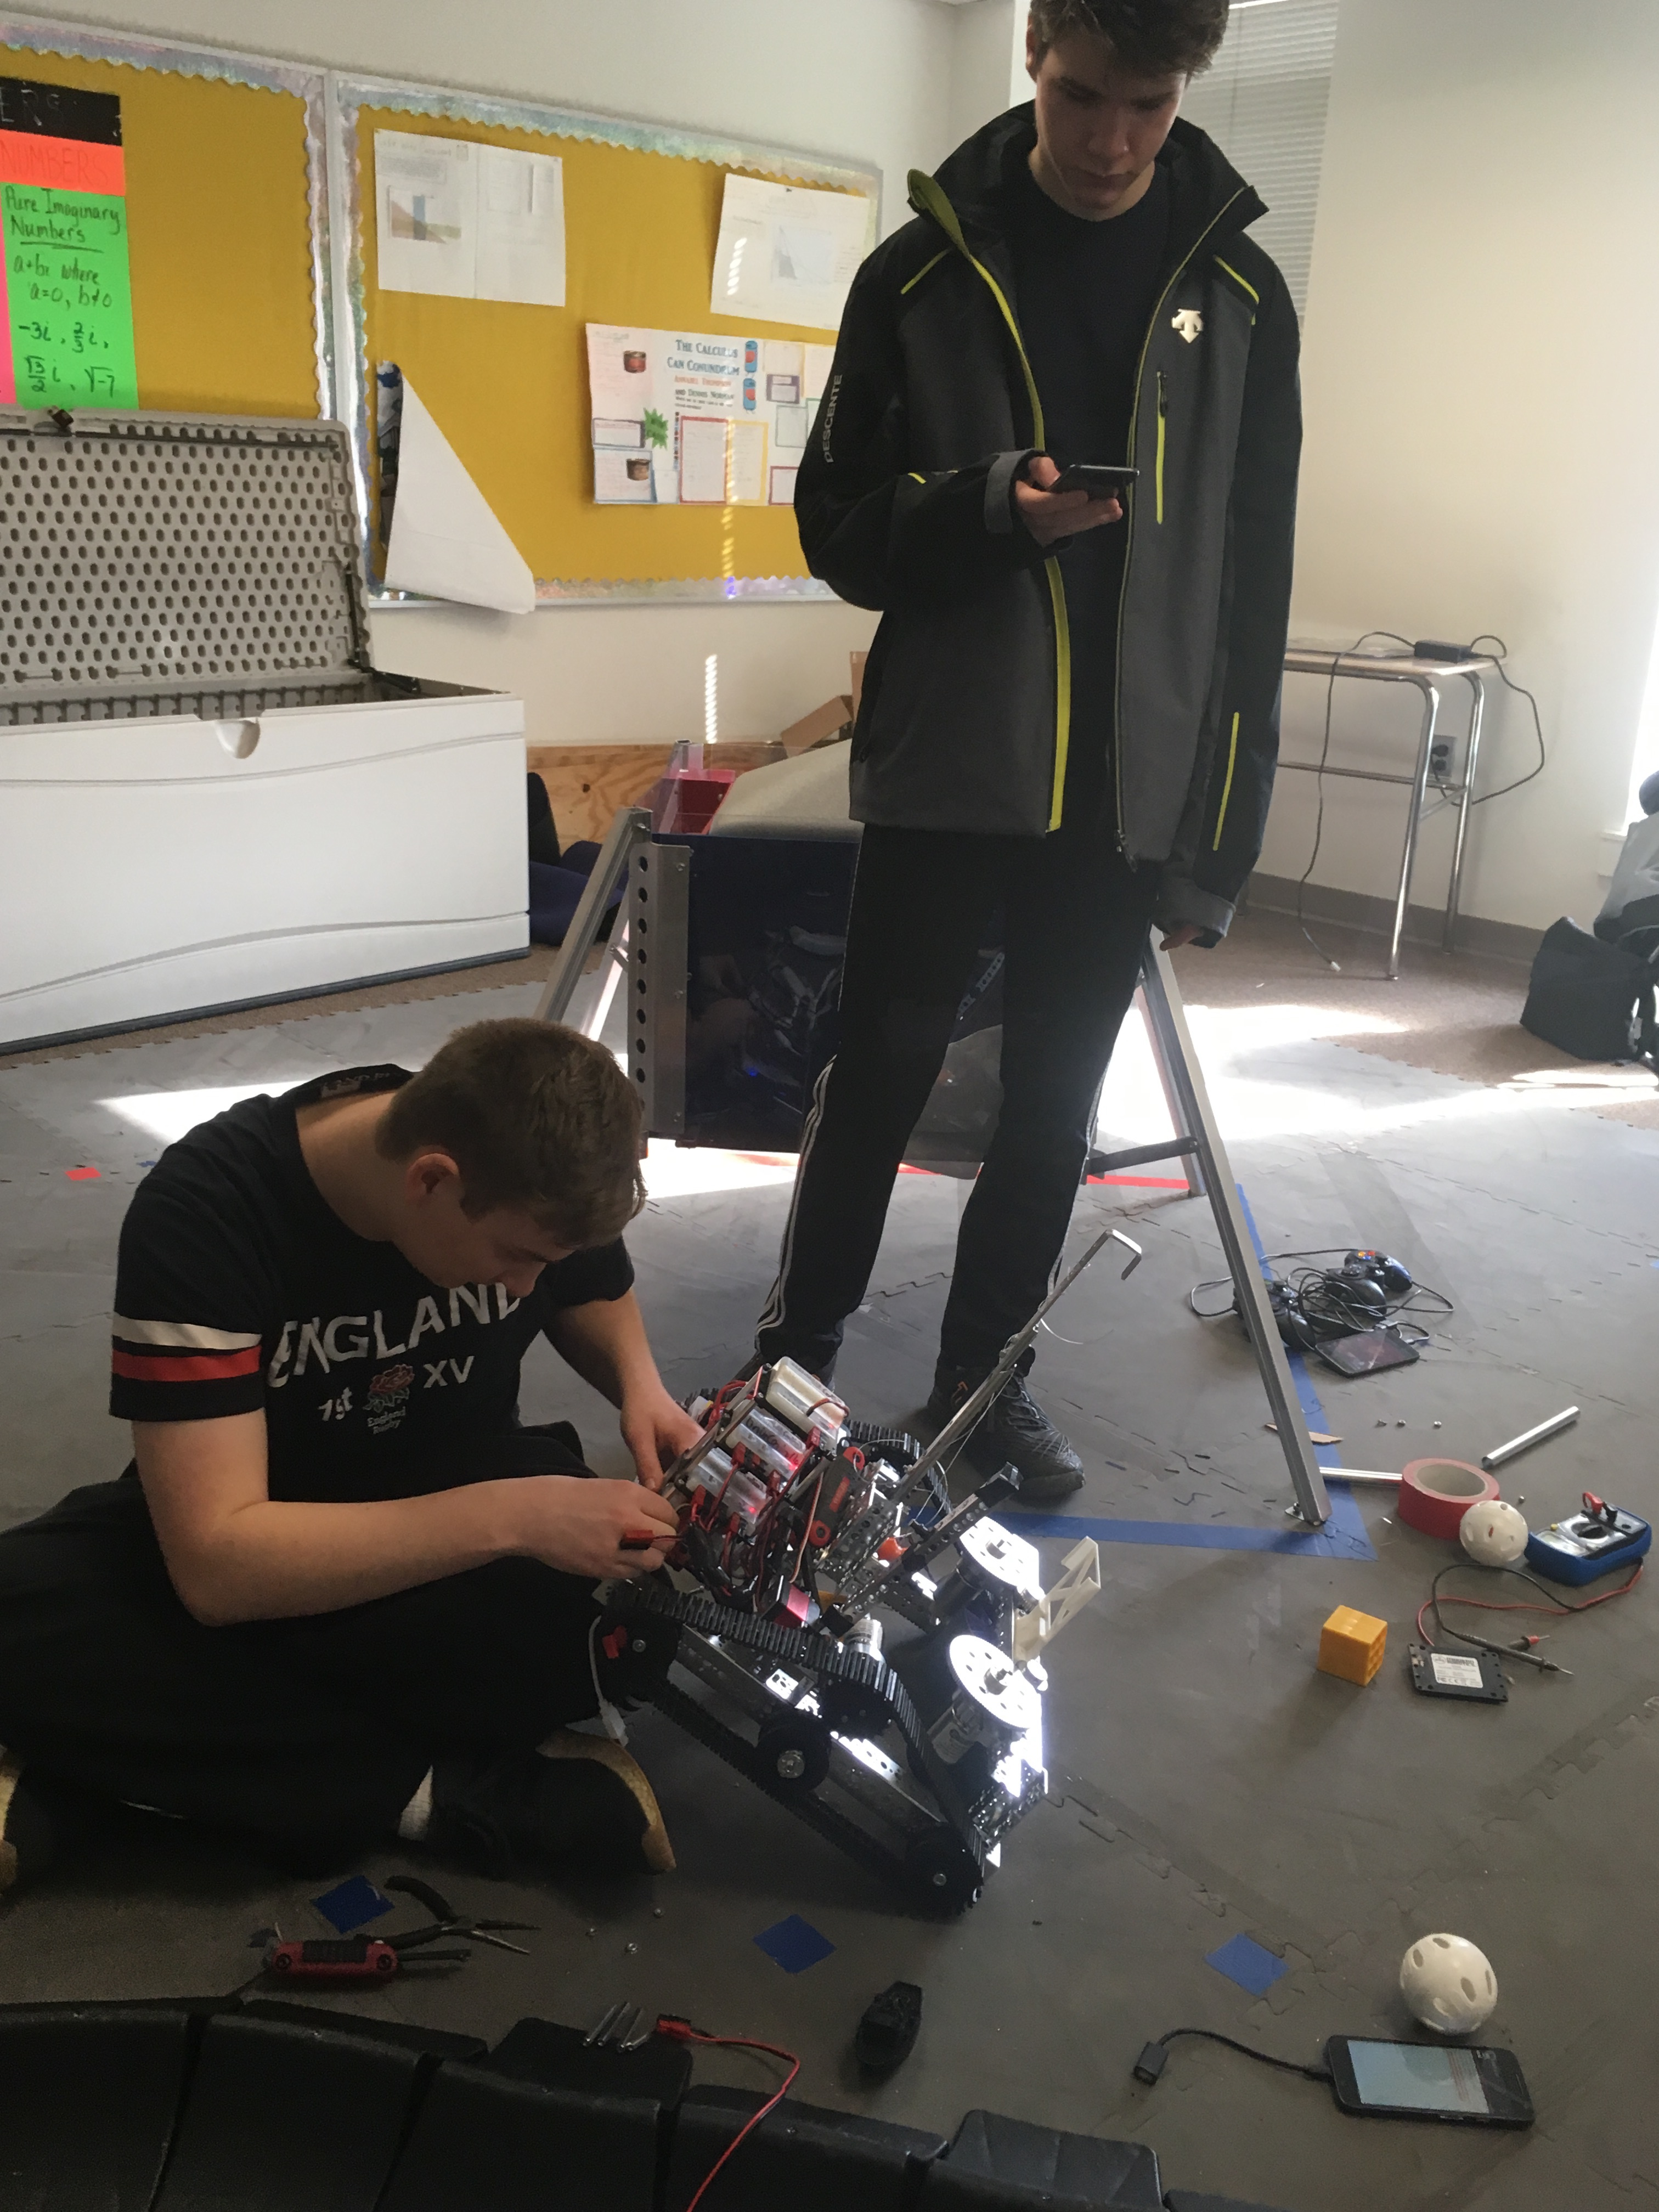
\includegraphics[width=75mm,scale=0.5]{jan5/IMG_3672}
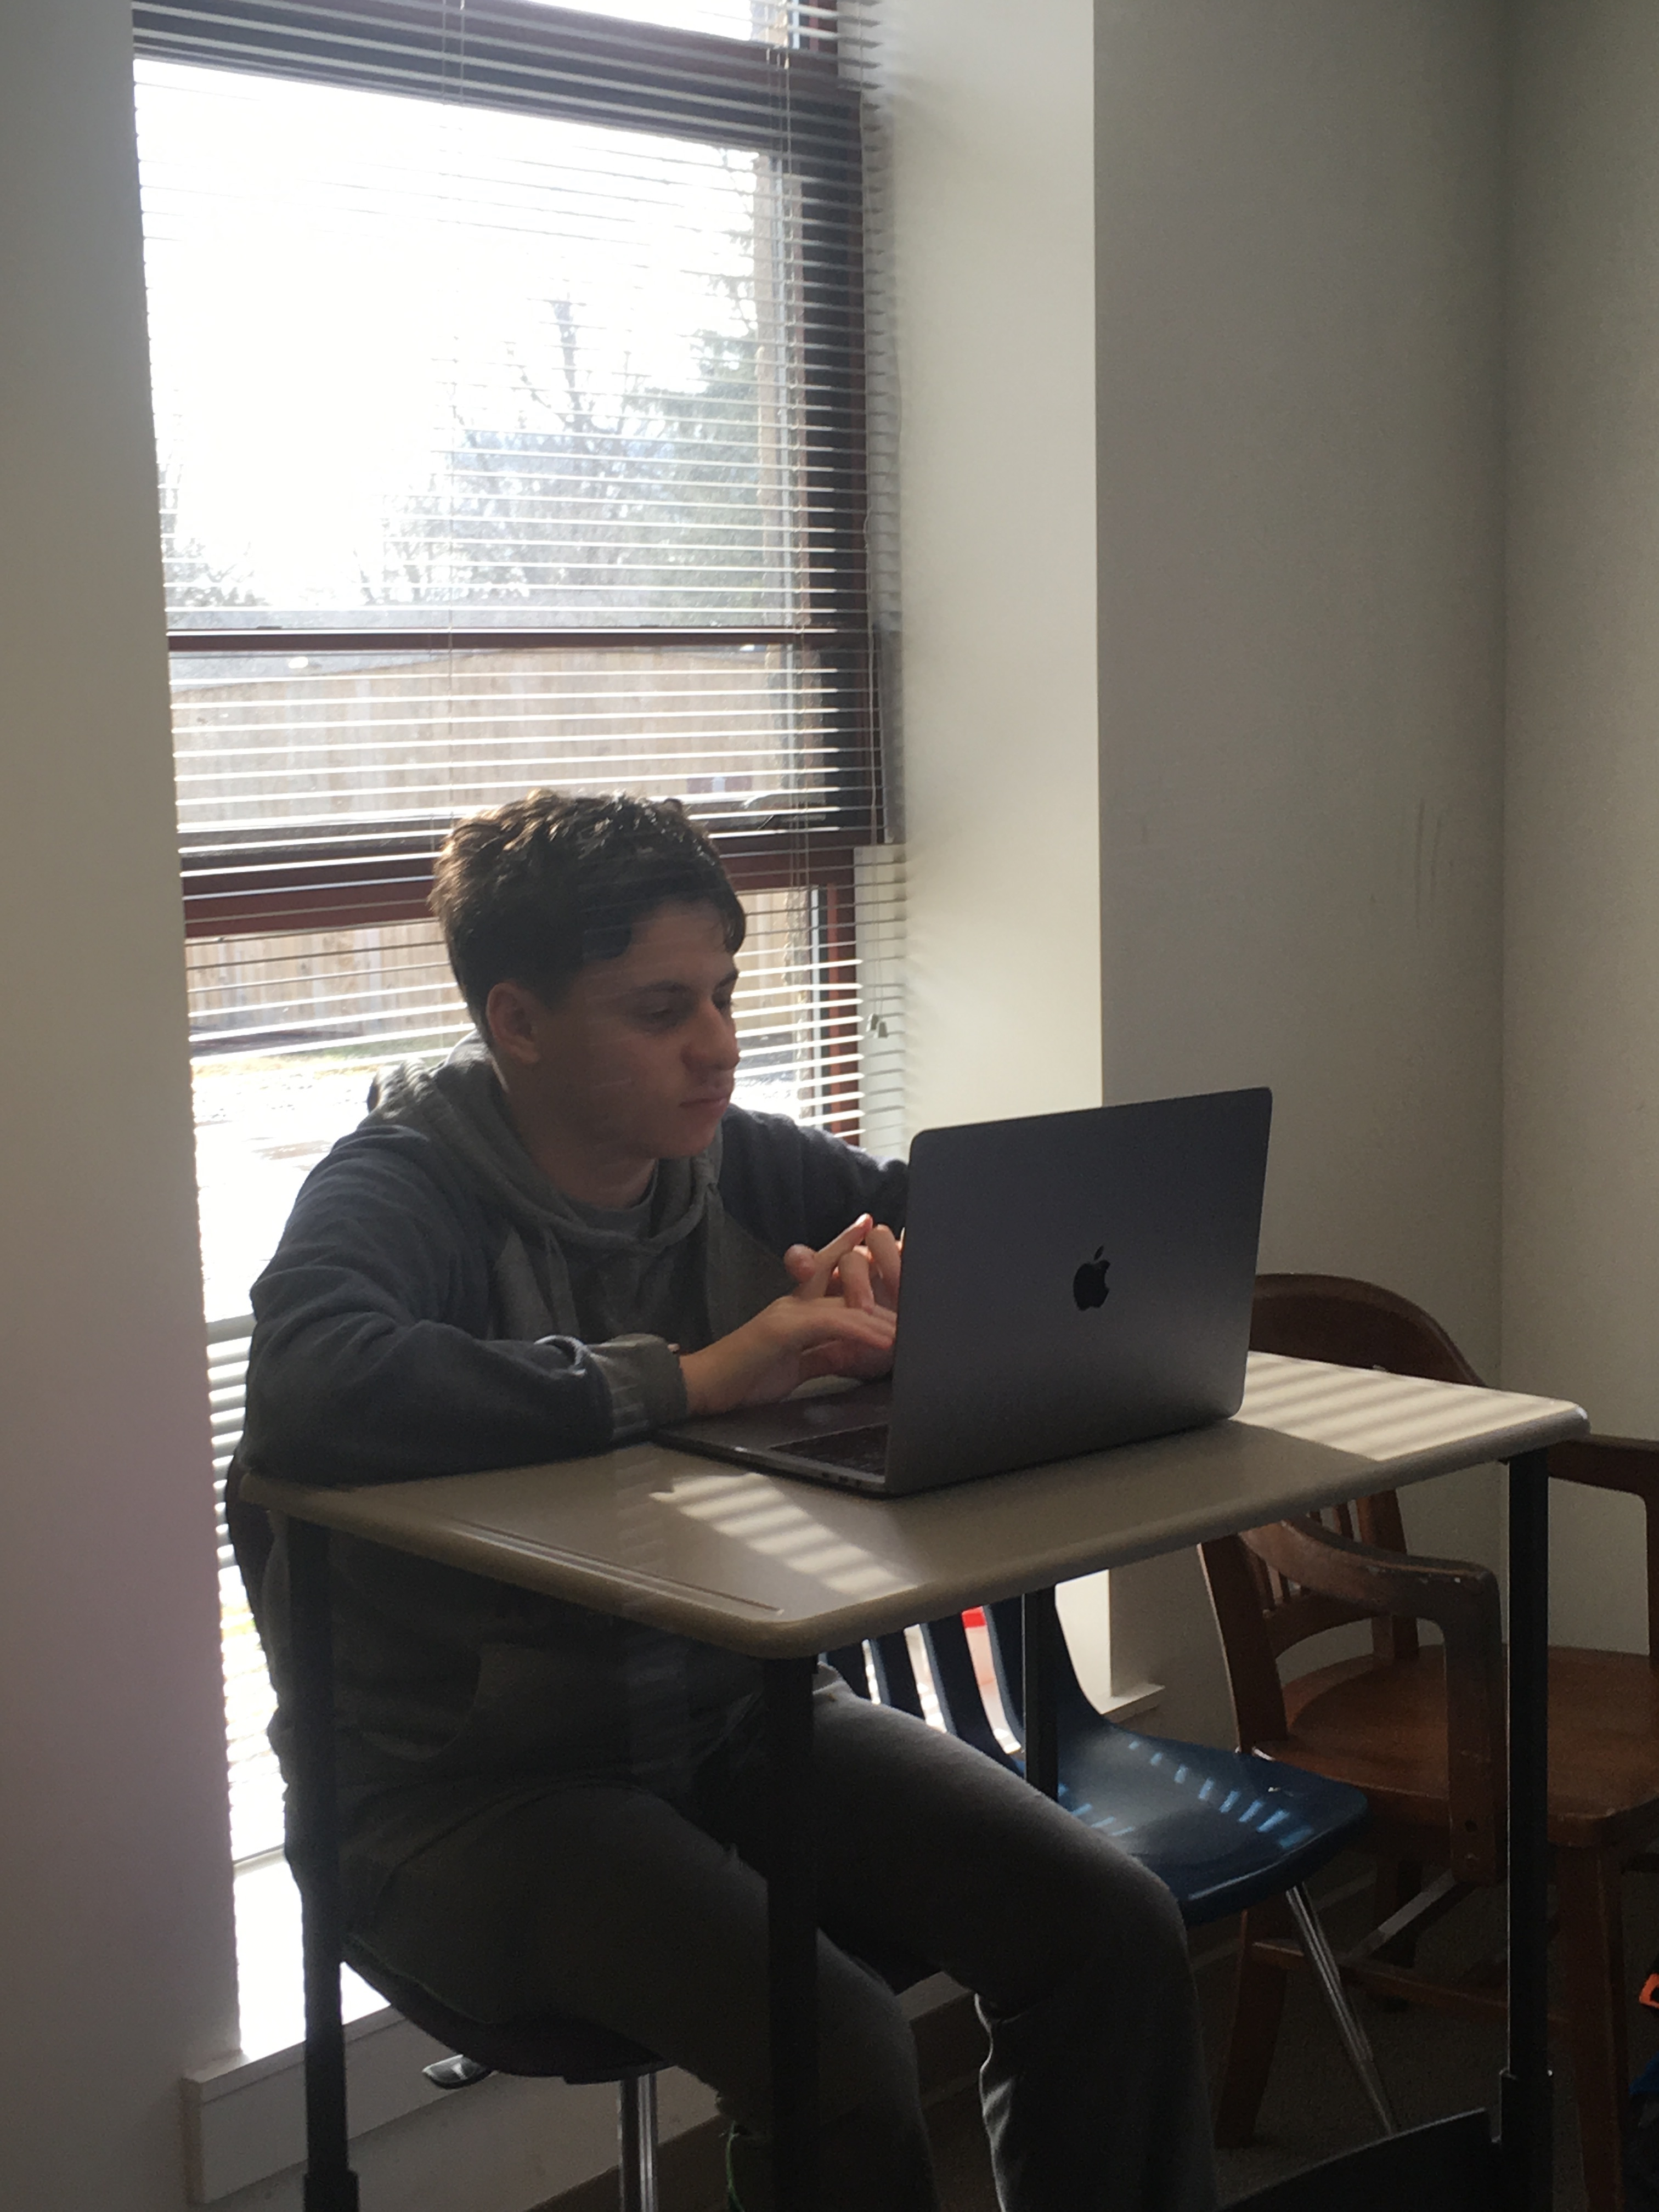
\includegraphics[width=75mm,scale=0.5]{jan5/IMG_3666}

\newpage
\setcounter{section}{0}

January 6th, 2019 - Griffin Dugan

\section{Our Plan:}
\begin{itemize}
	\item we plan to restring the Stronk Boi
	\item fine tune autonomous to sense the orientation images in the arena and move better
	\item fix code
	\item work on mineral holding device
\end{itemize}

We plan to restring the stronk boi with Paracord. We want to fine tune the autonomous so that it can move through the field much better. We need to fix the code. We also need to work on the mineral holding device.

\section{What we did:}
\begin{itemize}
	\item Restrung the stronk boi
	\item Worked on fine tuning the autonomous
	\item Worked on mineral holding device
\end{itemize}

This practice, we were able to restring the stronk boi with Paracord, now it works a lot better. We worked on fine tuning the autonomous, but it's not completely perfect currently. W also attempted to add the mineral holder, but we weren't able to add it fully quite yet due to us not having sides to the holder.

\section{What we didn't do:}
\begin{itemize}
	\item Fix code
\end{itemize}

We weren't able to fully fix the code yet. We had a few errors happen, like a servo start smoking. We still need to work on fixing the code.

\section{Next Practice:}
\begin{itemize}
	\item Add sides for the mineral picker.
	\item Finish code
	\item Get ready for the competition.
\end{itemize}

Our next practice is on Friday the 11th of January. We need to get the robot completely working since we have our first competition the day after this next practice. We need to make sure that everything is working well \textit{enough}. Hopefully, it will go well.

\newpage
\setcounter{section}{0}
\setcounter{page}{91}










\section*{Website}

\section{Website Proposal}
The Key School Robotics Team wishes to buy a domain in order to host our robotics website. This website is created and maintained by the robotics team. Nothing will be placed on the website without permission from Derek. We plan to promote our team to other teams or to sponsors. Currently, we have no logos of the Key School on the website, but we hope to add a logo if this is approved.

\section{Photos of Our Website}

\includegraphics[width=150mm,scale=0.5]{website/2019-01-06_1037.png}

\newpage
\setcounter{section}{0}
\setcounter{page}{101}

\begin{table}[]
\caption{The Parts List}
\label{Parts List}
\begin{tabular}{lll}
\rowcolor[HTML]{6665CD} 
Part Name & Part Number & Quantity \\
\rowcolor[HTML]{FFCC67} 
STRUCTURAL COMPONENTS & - & - \\ \hline
TETRIX 120 tooth aluminum gears & W39085 & 2 \\
TETRIX 40 tooth aluminum gears & W39028 & 2 \\
TETRIX MAX 96mm Channels & W39066 & 3 \\
TETRIX MAX 416mm Channels & W39069 & 2 \\
TETRIX MAX 288mm Channels & W39068 & 3 \\
TETRIX MAX 4.7 mm Axle 100mm & W39088 & 14 \\
Socket Head Cap Screw 1-1/2" & W39195 & 4 \\
Socket Head Cap Screw 1/2" & W39097 & Several \\
Socket Head Cap Screw 5/16" & W39098 & Several \\
TETRIX MAX 12-Volt Rechargeable Battery Pack & W39057 & 2 \\
TETRIX MAX Tank Tread Kit & W36468 & 1 \\
TETRIX MAX Worm Gear Box & W39375 & 1 \\
TETRIX MAX 11 mm Bronze Bushing & W39091 & Several \\
Kep Nut & W39094 & Several \\
Quarter-Scale HS-785HB Winch Servo Motor with Horn & W39905 & 1 \\
TETRIX MAX Axle Hub & W39172 & 9 \\
TETRIX MAX DC Motor & W39530 & 5 \\
TETRIX MAX DC Motor Mount & W39376 & 5 \\
TETRIX MAX L Bracket & W39062 & 2 \\
TETRIX MAX Motor Power Cable & W31903 & 5 \\
TETRIX MAX Inside Corner Bracket & W39281 & 2 \\
TETRIX MAX Single Standard-Scale Servo Motor Bracket & W39060 & 1 \\
TETRIX PRIZM On/Off Switch Kit & W43169 & 1 \\
TETRIX MAX DC Motor Expansion Controller & W44354 & 3 \\
TETRIX MAX Servo Motor Expansion Controller & W44355 & 1 \\
TETRIX PRIZM Robotics Controller & W43000 & 1 \\
THK Single Slide Rail & FBL35S & 1 \\
TETRIX MAX Flat Bar & W39070 & 1 \\
TETRIX MAX Inside C Connector & W39270 & 2 \\
TETRIX PRIME Square Beams & W40205 & 1 \\
TETRIX PRIME Beam End Connectors & W40214 & 1 \\
\rowcolor[HTML]{FFCC67} Other & - & - \\ \hline
TPU 3D Printing Filament & - & - \\
PLA 3D Printing Filament & - & - \\
Moto G Play Phones & - & 2 \\
\end{tabular}
\end{table}



















\end{document}